\documentclass[draft,grl]{agutexSI2019}

\usepackage{graphicx}
\setkeys{Gin}{draft=false}

\authorrunninghead{RAUPACH AND ALDRIDGE}
\titlerunninghead{CHANGES IN DAMAGING HAIL IN AUSTRALIA}

\authoraddr{Corresponding author: T. H. Raupach,
UNSW Sydney Climate Change Research Centre,
Mathews Building Level 4, 
UNSW Sydney, 
New South Wales 2052,
Australia
(timothy.h.raupach@gmail.com)}

\begin{document}

\title{Supporting Information for ``Changes in damaging hail in major Australian cities with global warming''}
% % %DOI: 10.1002/%insert paper number here%

\authors{Timothy H. Raupach\affil{1,2,3}, Joanna Aldridge\affil{4,5}}

\affiliation{1}{UNSW Institute for Climate Risk and Response, 
                UNSW Sydney, New South Wales, Australia}
\affiliation{2}{UNSW Climate Change Research Centre, 
                UNSW Sydney, New South Wales,  Australia}
\affiliation{3}{ARC Centre of Excellence for Climate Extremes, 
                Sydney, New South Wales,  Australia}
\affiliation{4}{School of Geosciences, University of Sydney, 
                Sydney, New South Wales,  Australia}
\affiliation{5}{QBE Australia, Sydney, 
                New South Wales, Australia}

\begin{article}

\noindent\textbf{Contents of this file}
\begin{enumerate}
    \item Figures S1 to Sx.
    \item Tables S1 to Sx.
\end{enumerate}

\clearpage

\bibliography{../main/library}

\end{article}

% % \clearpage

\begin{figure}[!h]
    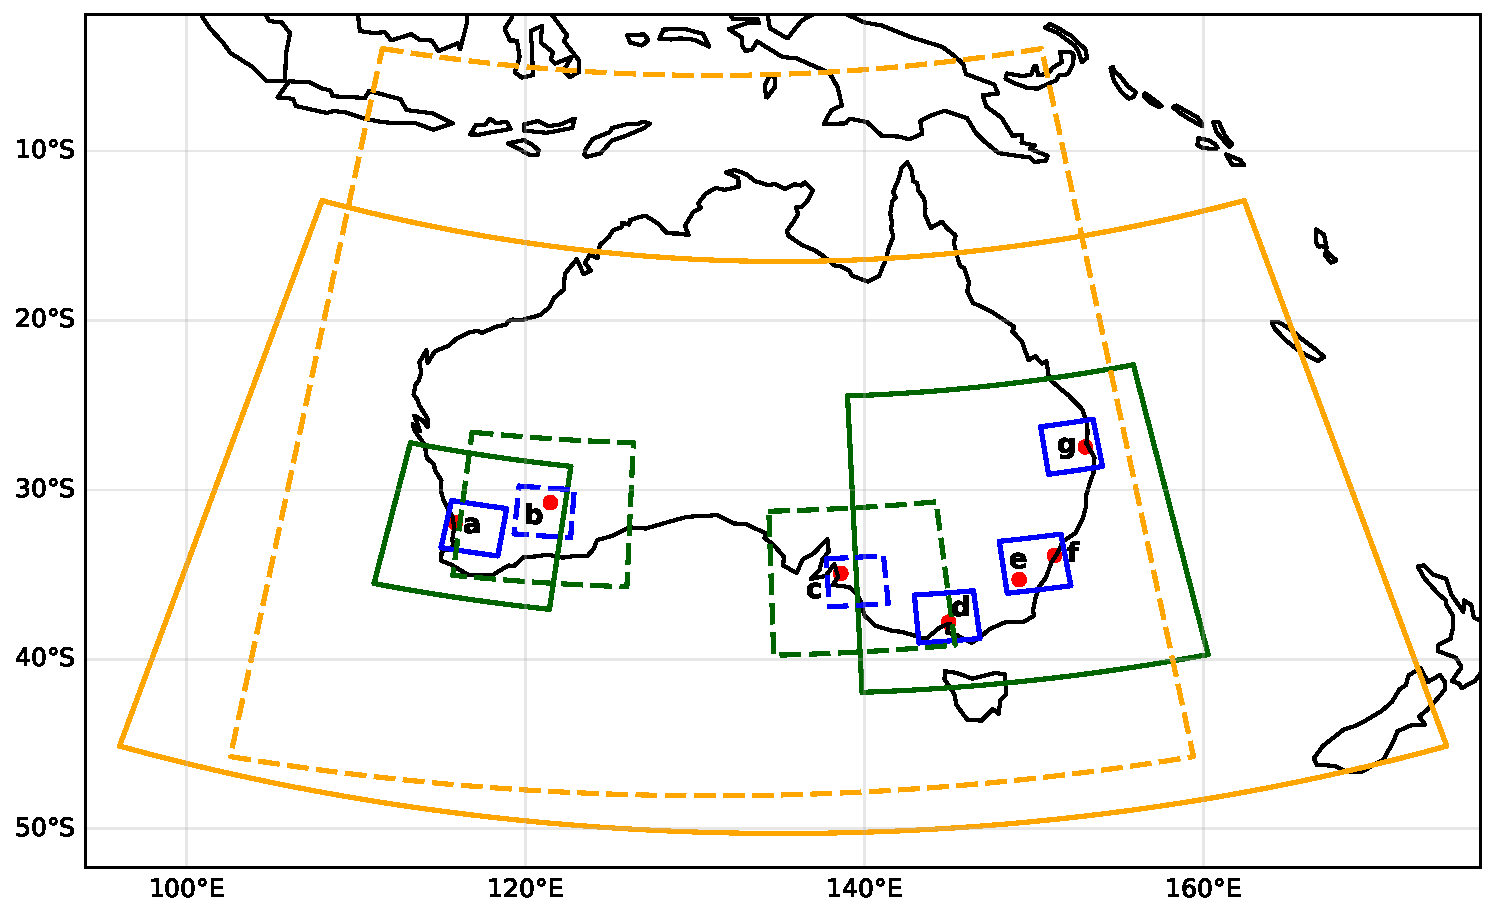
\includegraphics[width=\textwidth]{figures/domains}
    \caption{Approximate extents of the model domains on a map of Australia. The coarse-resolution domains are in yellow, medium-resolution domains in dark green, and fine-resolution domains in blue. The solid and dotted lines group the two sets of nested domains that were calculated together. Approximate city locations (with city extents not shown) are marked with red points for Perth (a), Kalgoorlie (b), Adelaide (c), Melbourne (d), Canberra (e), Sydney (f), and Brisbane (g).}
    \label{fig:domains}
\end{figure}

\end{document}

% % % Single-line equations are centered.
% % % Equation arrays will appear left-aligned.

% % Math coded inside display math mode \[ ...\]
% %  will not be numbered, e.g.,:
% %  \[ x^2=y^2 + z^2\]

% %  Math coded inside \begin{equation} and \end{equation} will
% %  be automatically numbered, e.g.,:
% %  \begin{equation}
% %  x^2=y^2 + z^2
% %  \end{equation}

% % % IF YOU HAVE MULTI-LINE EQUATIONS, PLEASE
% % % BREAK THE EQUATIONS INTO TWO OR MORE LINES
% % % OF SINGLE COLUMN WIDTH (20 pc, 8.3 cm)
% % % using double backslashes (\\).

% % % To create multiline equations, use the
% % % \begin{eqnarray} and \end{eqnarray} environment
% % % as demonstrated below.
% % \begin{eqnarray}
% %   x_{1} & = & (x - x_{0}) \cos \Theta \nonumber \\
% %         && + (y - y_{0}) \sin \Theta  \nonumber \\
% %   y_{1} & = & -(x - x_{0}) \sin \Theta \nonumber \\
% %         && + (y - y_{0}) \cos \Theta.
% % \end{eqnarray}

% % %If you don't want an equation number, use the star form:
% % %\begin{eqnarray*}...\end{eqnarray*}

% % % Break each line at a sign of operation
% % % (+, -, etc.) if possible, with the sign of operation
% % % on the new line.

% % % Indent second and subsequent lines to align with
% % % the first character following the equal sign on the
% % % first line.

% % % Use an \hspace{} command to insert horizontal space
% % % into your equation if necessary. Place an appropriate
% % % unit of measure between the curly braces, e.g.
% % % \hspace{1in}; you may have to experiment to achieve
% % % the correct amount of space.


% % %% ------------------------------------------------------------------------ %%
% % %
% % %  EQUATION NUMBERING: COUNTER
% % %
% % %% ------------------------------------------------------------------------ %%

% % % You may change equation numbering by resetting
% % % the equation counter or by explicitly numbering
% % % an equation.

% % % To explicitly number an equation, type \eqnum{}
% % % (with the desired number between the brackets)
% % % after the \begin{equation} or \begin{eqnarray}
% % % command.  The \eqnum{} command will affect only
% % % the equation it appears with; LaTeX will number
% % % any equations appearing later in the manuscript
% % % according to the equation counter.
% % %

% % % If you have a multiline equation that needs only
% % % one equation number, use a \nonumber command in
% % % front of the double backslashes (\\) as shown in
% % % the multiline equa
% % tion above.
